\subsection{Überblick}
\label{subsec:uberblick}

Der Canny-Algorithmus ist ein mehrstufiges Verfahren zur Kantendetektion in
Graustufenbildern. Canny definiert drei Kriterien für einen optimalen
Kantendetektor: gute Detektion, präzise Lokalisierung sowie exakt eine
Antwort pro Kante, die auf eine Breite von einem Pixel supprimiert werden
soll \cite[S.~680]{canny1986}. Die Verarbeitung erfolgt in vier aufeinanderfolgenden
Schritten, wobei der Output jedes Schritts als Input des nächsten dient
(siehe Abbildung~\ref{fig:pipeline}). Die einzelnen Schritte werden in den
kommenden Abschnitten näher erläutert.

\begin{figure}[h]
    \centering
    \resizebox{\textwidth}{!}{
        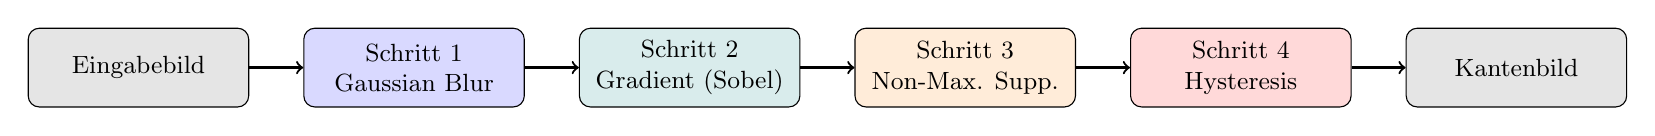
\begin{tikzpicture}[
            box/.style={rectangle, draw, rounded corners, minimum width=2.8cm,
            minimum height=1cm, align=center, font=\small},
            arrow/.style={->, thick}
        ]
            \node[box, fill=gray!20]   (input)  at (0,0)    {Eingabebild};
            \node[box, fill=blue!15]   (blur)   at (3.5,0)  {Schritt 1\\Gaussian Blur};
            \node[box, fill=teal!15]   (sobel)  at (7,0)    {Schritt 2\\Gradient (Sobel)};
            \node[box, fill=orange!15] (nms)    at (10.5,0) {Schritt 3\\Non-Max. Supp.};
            \node[box, fill=red!15]    (hyst)   at (14,0)   {Schritt 4\\Hysteresis};
            \node[box, fill=gray!20]   (output) at (17.5,0) {Kantenbild};

            \draw[arrow] (input)  -- (blur);
            \draw[arrow] (blur)   -- (sobel);
            \draw[arrow] (sobel)  -- (nms);
            \draw[arrow] (nms)    -- (hyst);
            \draw[arrow] (hyst)   -- (output);
        \end{tikzpicture}
    }
    \caption{Canny Edge Detection Pipeline}
    \label{fig:pipeline}
\end{figure}